\documentclass[1_relazione.tex]{subfiles}
\begin{document}

\section{Progettazione}
Questa sezione introduce la progettazione del sito. Per rendere pi\`{u} chiaro il documento, introduciamo prima gli elementi di progettazione e nella successiva sezione la realizzazione. Dove possibile, abbiamo sempre anticipato la progettazione alla realizzazione. Per esempio la scelta di usare un modello gerarchico per il sito, la struttura della home page e la presentazione dei risultati di ricerca in forma di lista sono stati scelti in anticipo. Per alcune parti del sito, progettazione e realizzazione sono andate in parallelo.

\subsection{Base di dati}
La prima fase della progettazione è stata la base di dati.  Il modello Entità-Relazione è stato utilizzato come punto di partenze per definire lo scopo e gli utilizzatori del sito. Per maggiore chiarezza, riportiamo sia lo schema ER che lo schema relazionale. La spiegazione approfondita è stata inserita nella precedente sezione, Scopo del sito.

\begin{figure}[h!]
\centering
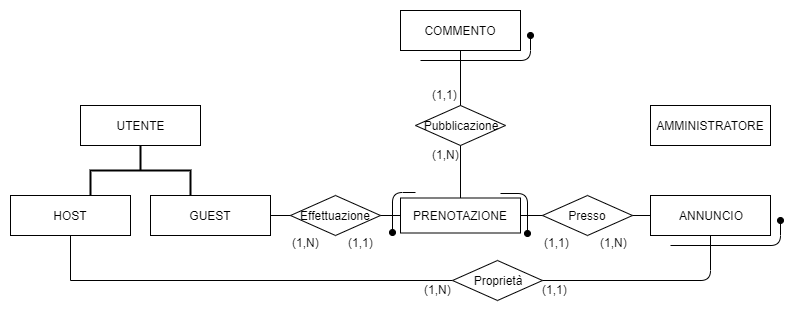
\includegraphics[scale=0.5]{immagini/schema_ER-2}
\caption{Schema ER}
\end{figure}

\begin{figure}[h!]
\centering
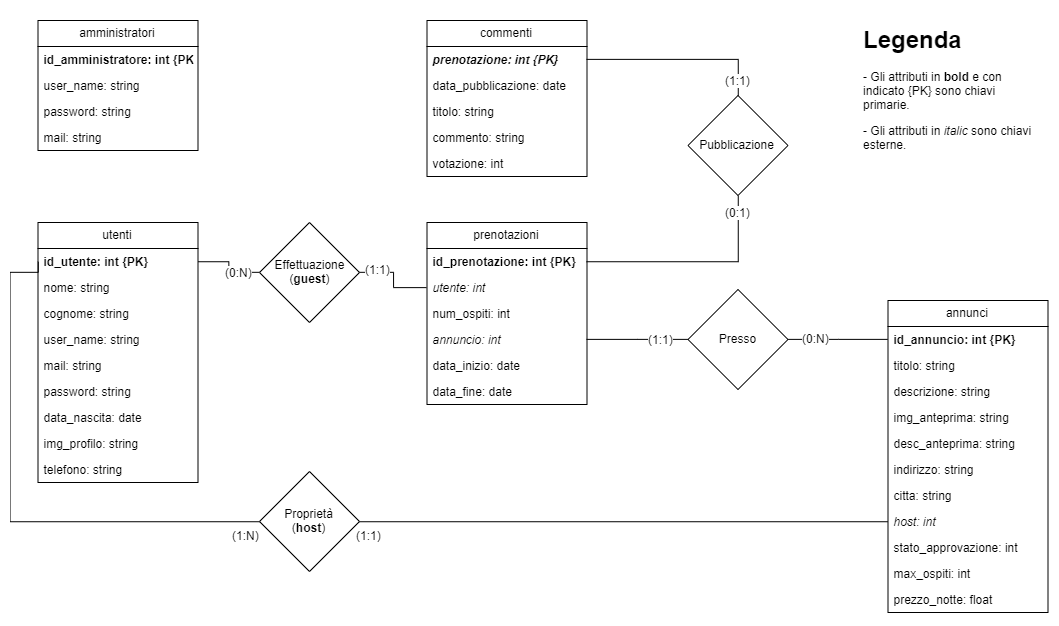
\includegraphics[scale=0.4]{immagini/schema_relazionale-2}
\caption{Schema relazionale}
\end{figure}

\subsubsection{Dati guest richiesti}
In questa fase abbiamo anche pensato a che informazioni chiedere all'utente per registrarsi a FRENT per non rendere i form troppo lunghi. La data di nascita è un requisito fondamentale per poter affittare/noleggiare un immobile ed è quindi obbligatorio inserirla. Un campo utile ma non strettamente necessario è il numero di telefono dell'utente. Per non complicare troppo la realizzazione tutti i campi sono stati resi obbligatori. Come sviluppo futuro si potrebbe demandare l'inserimento del numero di telefono ad un secondo momento.

\subsection{Contesto dell'informazione }
Una volta definiti gli utenti, abbiamo pensato a come facilitare il pi\`{u} possibile l'utilizzo del sito. Come scelta preliminare abbiamo localizzato gli utenti come cittadini italiani che cercano alloggi in Italia. Eventuali internazionalizzazioni sarebbero state troppo complesse da gestire. Abbiamo quindi pensato agli obbiettivi degli utenti di FRENT.  Il punto di partenza \`{e} quindi capire \textit{cosa} vogliono di utenti:

\begin{itemize}
\item Guest: fare una ricerca, gestire le prenotazioni.
\item Host: inserire un annuncio, gestire gli annunci.
\end{itemize}

A questo punto abbiamo definito \textit{dove} gli utenti possono trovare ciò di cui hanno bisogno. Abbiamo utilizzato la metafora della pesca vista a lezione per capire come offrire agli utenti una esperienza piacevole e ridurre al minimo la complessità delle ricerche. Questo ha fornito gli elementi di base per organizzare la home del sito. Tutte le altre pagine gravitano a partire da questa.

\subsubsection{Tiro Perfetto} 
Il tiro perfetto è la metafora per indicare gli utenti che sanno cosa stanno cercando. Per questo motivo nella home page del sito abbiamo inserito un form orizzontale per effettuare la ricerca di annunci che ne soddisfino i parametri. In questo modo la funzione di ricerca è immediatamente disponibile e gli utenti possono sia ottenere delle informazioni velocemente che sperimentare direttamente che tipo di servizi offre FRENT.
 
\subsubsection{Trappola per aragoste} 
Per catturare l'attenzione degli utenti che stanno esplorando il sito, abbiamo inserito nel corpo centrale della home una sezione con gli ultimi annunci pubblicati. Il destinatario di questa sezione è un utente che esplora il sito nei tempi morti o vuole capire che tipo di servizi offre. Gli annunci sono la base del servizio offerto da FRENT ed è bene che gli utenti siano familiari con la loro struttura. Se un utente clicca sull'immagine di un annuncio viene inviato direttamente all'annuncio selezionato. Lo scopo \`{e} far creare all'utente tramite l'esperienza diretta una mappa mentale dal sito da utilizzare per scopi futuri. \\
Questo vale sia per i guest che per gli host. I guest possono capire com'\`{e} strutturato un annuncio e che informazioni sono disponibili. Gli host possono capire com'\`{e} strutturato un annuncio e quindi risulter\`{a} pi\`{u} facile compilare i campi del form per l'aggiunta di un annuncio. \\
Un possibile sviluppo futuro potrebbe essere inserire nella home altre sezione simili, ad esempio gli annunci pi\`{u} votati o le offerte last minute.\\ Abbiamo inserito gli ultimi annunci approvati per fornire un incentivo agli host a pubblicare nuovi annunci. \\

\subsubsection{Boa di Segnalazione}
La boa di segnalazione serve per ritrovare elementi informativi utili. Le boe di segnalazione in FRENT sono raggruppate in due zone, header e footer. Entrambe cambiano per utente generico e utente registrato.

\begin{itemize}
\item \textbf{Header}
Per l'utente generico diamo subito la possibilit\`{a} di registrarsi o di accedere. Per l'utente registrato invece offriamo un cruscotto per la gestione completa delle informazioni.
\item \textbf{Footer}
Per tutti gli utenti, il footer riporta invece informazioni di carattere generale, come le condizioni di utilizzo del sito e le FAQ. Queste informazioni si trovano di solito nel footer e abbiamo deciso di inserirle in basso per non violare le convenzioni esterne di utilizzo del sito.  Solo per gli utenti non registrati e solo nella pagina home, \`{e} presente il link verso la pagina di accesso per l'amministratore. Si trova in una posizione poco visibile perch\`{e} diamo per scontato che l'amministratore sia un utente che conosce il sito e sa dove andare a cercarlo.
\end{itemize}


\subsection{Schema organizzativi}
A questo punto la domanda che ci siamo posti \`{e} \textit{come} presentare le informazioni agli utenti. Abbiamo organizzato l'elenco delle informazioni usando degli schemi esatti. Le funzioni che l'utente pu\`{o} utilizzare per manipolare tali dati sono state raggruppate con schemi orientati al compito.

\subsubsection{Schemi esatti}
Per la presentazione dei risultati di ricerca, elenco prenotazioni,  elenco annunci degli host e elenco annunci amministratori, la scelta che ci \`{e} sembrata pi\`{u} naturale \`{e} stata presentare le informazioni in modo esatto:

\begin{itemize}
\item \textbf{Ricerca}
La ricerca riporta l'elenco completo di tutti gli annunci che soddisfano le richieste dell'utente. \`{E} realizzato come un elenco in cui ogni elemento \`{e} strutturato allo stesso modo. In questo modo l'utente pu\`{o} farsi un'idea preliminare degli annunci disponibili. Cliccando su un annuncio si viene portati ad una nuova pagina che entra nel dettaglio delle informazioni.

\item\textbf{Elenco prenotazioni guest}
L'elenco prenotazioni riporta tutte le prenotazioni di un guest, raggruppate in base al loro tipo: passate, correnti e future. Ovviamente i risultati di questa pagina sono influenzati dalla data corrente. Le prenotazioni sono riportate in questo ordine, prima corrente, poi future e infine passate. L'ordine riflette il valore che abbiamo attributo all'informazione dal punto di vista del guest.
\begin{enumerate}
\item \textbf{Corrente} L'informazione sulla prenotazioni corrente \`{e} stata giudicata la pi\`{u} importata e viene quindi presentata per prima. L'idea \`{e} che un utente in viaggio voglia controllare i dettagli della prenotazione o contattare l'host in modo rapido. Ad esempio vuole controllare l'indirizzo esatto mentre si sta viaggiando. Per questo motivo \`{e} stato inserito anche un pulsante per contattare l'host. Per semplicit\`{a} \`{e} il solo invio di una email.
\item \textbf{Future} Le prenotazioni future sono messe in seconda posizione perch\`{e} \`{e} probabile che l'informazione venga visualizzata frequentemente dall'utente mentre organizza viaggi.
\item \textbf{Passate} Le presentazioni passate sono messe alla fine perch\`{e} svolgono una funzione di storico per il guest e  per effettuare i commenti. \`{E} difficile che un utente vada regolarmente a controllare le prenotazioni passate e una volta lasciato il commento non ha pi\`{u} motivi specifici per tornare ad una vecchia prenotazione.
\end{enumerate}

\item \textbf{Elenco annunci host}
L'elenco degli annunci riporta gli annunci pubblicati da un host. In questo modo l'host pu\`{o} controllare in modo semplice tutti i propri annunci e il loro stato di approvazione. Sotto il titolo dell'annuncio viene riportato se l'annuncio \`{e} stato visualizzato e/o approvato dall'amministratore. Inoltre \`{e} presente un pulsante per andare ad un pagina specifica per la gestione del singolo annuncio.

\item \textbf{Prenotazioni annuncio} Questo campo \`{e} analogo all'elenco prenotazioni per il guest, ma elenca tutte le prenotazioni dell'annuncio.

\item \textbf{Elenco annunci da approvare}
L'elenco degli annunci da approvare offre all'amministratore tutti gli annunci che devono essere verificati. 

\end{itemize}

\subsubsection{Schemi ambigui}
Le funzioni per manipolare i dati sono specifiche e sono state organizzati in schemi orientati al compito. In questo modo l'utente ha un'indicazione precisa su dove andare per eseguire le operazioni.

\begin{itemize}
\item \textbf{Header utenti registrati}
\begin{itemize}
\item \textbf{Le mie prenotazioni} I guest possono visualizzare le informazioni sulle loro prenotazioni.
\item \textbf{I miei annunci} Per gestire gli annunci e inserirne di nuovi. Gli host possono controllare tutti i propri annunci. Inoltre viene ben evidenziata l'opzione "Nuovo Annuncio" per permettere agli utenti di creare un nuovo annuncio.
\item \textbf{Il mio profilo} Visualizzazione e modifica dei dati del profilo. 
\end{itemize}

\item \textbf{Gestione annunci host}
\begin{itemize}
\item \textbf{Modifica} Modifica le informazioni relative ad un annuncio.
\item \textbf{Prenotazioni} Tutte le prenotazioni relative ad un singolo annuncio.
\item \textbf{Elimina Annuncio} Permette di eliminare un annuncio e avvisa se sono presenti prenotazioni correnti e future.
\end{itemize}
\end{itemize}

\subsection{Struttura organizzativa}
Le pagine di FRENT sono organizzate in modo gerarchico. La pagina di partenza \`{e} la home da cui \`{e} possibile raggiungere tutte le principali funzioni del sito. Per ciascun livello si \`{e} cercato di elencare funzioni mutualmente esclusive. Ad esempio la home porta alle pagine "Le mie prenotazioni" e "I miei annunci" per gestire prenotazioni e annunci. Inoltre le relazioni padre-figlio fra pagine sono state pensate per essere naturali. Ad esempio dalla pagina "I miei annunci" si arriva all'elenco degli annunci pubblicati da un host. Per ciascun annuncio si pu\`{o} andare alla pagina per la sua gestione che riporta tutte le funzioni specifiche per il singolo annuncio.\\In modo analogo, la pagina "Le mie prenotazioni" riporta tutte le prenotazioni fatte dal guest. Per ciascuna prenotazione si pu\`{o} andare a vederne i dettagli. \\
Per motivi di semplicit\`{a} FRENT utilizza alcuni elementi di ipertesto. Le pagine di "Accesso" e "Registrazione" sono collegate fra di loro. In questo modo un utente che sbaglia ad accedere ad una funzione (ad esempio un utente non registrato prova a fare l'accesso) può sempre raggiungere la pagina alla quale era interessato. La pagina FAQ rimanda alla pagine del sito che trattano la domanda trattata. \\
La pagina per i dettagli di un annuncio che un host pu\`{o} visualizzare \`{e} la stessa dei risultati di ricerca. In questo modo l'host pu\`{o} vedere la pagina come appare ad un guest dopo la ricerca; in questo caso le funzioni per effettuare la prenotazione non vengono visualizzate (un host non pu\`{o} essere guest di se stesso). Inoltre vi \`{e} un pulsante che permette di andare alla pagina per la modifica dei dati dell'annuncio.

\subsection{Web design}
Per impostare il layout delle pagine abbiamo cercato di utilizzare degli schemi quanto pi\`{u} semplici possibile. Per aiutare la navigazione tutte le pagine riportano il breadcrumb con il percorso completo per arrivare alla pagina. In questo modo l'utente pu\`{o} ricostruire in maniera intuitiva il percorso che ha fatto.\\ Per non creare confusione, nei menu con link non abbiamo inserito link circolari. \\
Per organizzare le pagine abbiamo utilizzato un interfaccia a schede e un layout a tre pannelli per alcune pagine.

\subsubsection{Interfaccia a schede} 
Le pagine sono organizzate con interfaccia a schede che rispetta la gerarchia. Sono presenti della etichette con dei link che permettono di navigare il sito e raggiungere tutte le componenti principali.
\subsubsection{Layout a tre pannelli} 
Per la pagina con i risultati delle ricerca e gestione annuncio abbiamo utilizzato un layout a tre panelli. L'header \`{e} lo stesso delle pagine con interfaccia a schede. Il menu laterale cambia per offrire un supporto specifico per la pagina.

\begin{itemize}
\item \textbf{Risultati di ricerca} Il men\`{u} laterale riassume i parametri utilizzati dall'utente per la ricerca e la possibilit\`{a} di fare nuove ricerche. In questo modo l'utente non deve tornare alla home per eseguire una nuova ricerca (ad esempio se non ci sono risultati o ha inserito i campi in modo sbagliato).
\item \textbf{Gestione annuncio} Il menu laterale riporta tutte le funzioni per gestire un annuncio. 
\end{itemize}

\subsection{Mobile}
L'accorgimento principale per la versione mobile è la riorganizzazione delle comnponenti della pagina.\\
\begin{itemize}
    \item \`{E} Stato eliminato il breadcrumb per dare maggior spazio alle altre informazioni.
    \item Il menù è stato spostato in fondo alla pagina e viene visualizzato un pulsante in alto a destra, in modo da essere facilmente raggiungibile con il pollice. Tale pulsante è un link al menù.
\end{itemize}



\subsection{Emozioni}
Abbiamo cercato di introdurre alcune componenti emotive nella realizzazione del sito.

\begin{itemize}
\item \textbf{Commenti} Per coinvolgere l'utente, abbiamo deciso di dare la possibilit\`{a} di esprimere la propria opinione sulla prenotazione e dare un voto. Per dare rilevanza, i commenti sono inseriti sotto i dettagli dell'annuncio. Per semplicit\`{a}, non ci sono funzioni di moderatore e i commenti non possono essere segnalati.

\item \textbf{Buon compleanno} Come forma di sorpresa, inseriamo gli auguri di buon compleanno all'utente nell'header della pagina. Tra le informazioni che dobbiamo necessariamente raccogliere c'e' anche la data di nascita e quindi possiamo usarla per questo scopo.  

\item \textbf{Pagina 404} Abbiamo personalizzato la pagina 404 nel caso in cui l'utente faccia una ricerca con un l'id non presente. Gli annunci possono essere rimossi e quindi è possibile che una ricerca salvata fra i siti preferiti dall'utente non sia disponibile in futuro. L'obbiettivo è evitare che l'utente lasci la pagina, ad esempio per rabbia o frustrazione. Abbiamo inserito un'immagine per aiutare l'utente a capire cosa è successo e messaggio di avviso che fornisce un aiuto immediato.

\end{itemize}

Fra le emozioni che si possono sfruttare per sviluppi futuri sono la reward e l'esclusivit\`{a}. Come reward si possono inserire sconti ed offerte per gli utenti di lungo periodo. Come esclusivit\`{a} avevamo pensato ad inserire una forma di status per il guest sulla base del numero di prenotazioni fatte. Le prenotazioni possono essere associate ai viaggi e l'utente riceverebbe uno status come ad esempio "Viaggiatore Esperto" o "Viaggiatore di Livello X". Questo campo verrebbe visualizzato nei commenti e nel profilo dell'utente.

\end{document}